\chapter[NIPTeR: an R package for NIPT analysis]{NIPTeR: an R package for fast and accurate trisomy prediction in non-invasive prenatal testing}
\chaptermark{NIPTeR: an R package for NIPT analysis}
\label{chap:NIPTeR}

{ \Large \leftwatermark{
		\put(-67,-66.5){ 1 }
		\put(-67,-91.5){ 2 }
		\put(-67,-116.5){ 3 }
		\put(-67,-141.5){ 4 }
		\put(-67,-166.5){ 5 }
		\put(-67,-191.5){ 6 }
		\put(-76.5,-225){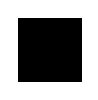
\includegraphics[scale=0.8]{img/thumbindex.eps}} \put(-67,-216.5){ {\color{white} 7 }}
		\put(-67,-241.5){ 8 }
		\put(-67,-266.5){ 9 }
		\put(-67,-291.5){ 10 }
		\put(-67,-316.5){ 11 }
	} \rightwatermark{
		\put(350.5,-66.5){ 1 }
		\put(350.5,-91.5){ 2 }
		\put(350.5,-116.5){ 3 }
		\put(350.5,-141.5){ 4 }
		\put(350.5,-166.5){ 5 }
		\put(350.5,-191.5){ 6 }
		\put(346.5,-225){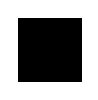
\includegraphics[scale=0.8]{img/thumbindex.eps}} \put(350.5,-216.5){ {\color{white} 7 }}
		\put(350.5,-241.5){ 8 }
		\put(350.5,-266.5){ 9 }
		\put(350.5,-291.5){ 10 }
		\put(350.5,-316.5){ 11 }
}}

\hfill \underline{BMC Bioinformatics} 2018;19:531.

\hfill DOI: \href{https://doi.org/10.1186/s12859-018-2557-8}{10.1186/s12859-018-2557-8}

\hfill PubMed ID: \href{https://www.ncbi.nlm.nih.gov/pubmed/30558531}{30558531}

\newpage

\noindent
L.F. Johansson\textsuperscript{1,2}, H.A. de Weerd\textsuperscript{1,2,3}, E.N. de Boer\textsuperscript{1}, F. van Dijk\textsuperscript{1,2}, G.J. te Meerman\textsuperscript{1}, R.H. Sijmons\textsuperscript{1}, B. Sikkema-Raddatz\textsuperscript{1}, M.A. Swertz\textsuperscript{1,2}\\

\noindent
1. University of Groningen, University Medical Center Groningen, Department of Genetics, Groningen, The Netherlands\\
2. University of Groningen, University Medical Center Groningen, Genomics Coordination Center, Groningen, The Netherlands\\
3. School of Bioscience, Systems biology research center, University of Skövde, Skövde, Sweden\\

\noindent
Received 2018 Oct 2; Accepted 2018 Dec 4; Published online 2018 Dec 17.
\\~\\


\section*{Abstract}\label{abstract}
\textbf{Background}
Various algorithms have been developed to predict fetal trisomies using cell-free DNA in non-invasive prenatal testing (NIPT). 
As basis for prediction, a control group of non-trisomy samples is needed. Prediction accuracy is dependent on the characteristics of this group and can be improved by reducing variability between samples and by ensuring the control group is representative for the sample analyzed.

\textbf{Results}
NIPTeR is an open-source R Package that enables fast NIPT analysis and simple but flexible workflow creation, including variation reduction, trisomy prediction algorithms and quality control. This broad range of functions allows users to account for variability in NIPT data, calculate control group statistics and predict the presence of trisomies.

\textbf{Conclusion}
NIPTeR supports laboratories processing next-generation sequencing data for NIPT in assessing data quality and determining whether a fetal trisomy is present. NIPTeR is available under the GNU LGPL v3 license and can be freely downloaded from \sloppy{https://github.com/molgenis/NIPTeR} or CRAN.


\section{Background}\label{Background}
Non-invasive prenatal testing (NIPT) is rapidly becoming the new standard in prenatal screening for fetal aneuploidy \cite{Allyse_2015}. 
In NIPT, cell-free DNA from the pregnant woman’s blood plasma, which consists of both maternal and fetal DNA fragments, is analysed. 
Next to SNP-based methods \cite{Hall_2014}, low-coverage whole genome next-generation sequencing (NGS) is often used \cite{Chiu_2008,Sehnert_2011}, and various algorithms, software programs and packages have been developed to analyse this type of data \cite{Chen_2011b, Straver_2013, Yang_2017, Sauk_2018, Phan_2018}. 
In literature, many methods have been described that depend on a statistical comparison between a sample of interest and a reference set of non-trisomy control samples \cite{Chiu_2008,Sehnert_2011,Fan_2010,Johansson_2017}. 
The RAPIDR and DASAF R packages, for instance, have been described \cite{Lo_2014,Liu_2016} and they made several of these algorithms available, including GC-correction, the standard Z-score and the Normalized Chromosome Value (NCV), to create an analysis workflow in R. 
However, those packages lack features like chi-squared-based variation reduction ($\chi$2VR), regression-based Z-score (RBZ) and Match QC. 
These are all algorithms that we have extensively discussed before \cite{Johansson_2017}. 
In short, $\chi$2VR detects chromosomal regions that have a higher variability than expected by chance and reduces their weight so that, after correction, they have less impact on the fraction of reads mapped to the different chromosomes. 
The RBZ is an alternative Z-score calculation based on stepwise regression with forward selection. 
In the RBZ positive or negative correlation between chromosomal fractions is used to predict the number of reads to map onto the chromosome of interest if no trisomy is present. 
The Match QC score is a sum-of-squares-based approach to compare chromosomal fractions between the test sample and controls, and it provides a measure by which to determine whether a control group is representative for a specific sample. 
Here we report NIPTeR, an R package that provides fast NIPT analysis for research and diagnostics and provides users with multiple methods for variation reduction, prediction and quality control based upon comparison of a sample with a set of negative control samples.

\section{Implementation}\label{Implementation}
NIPTeR users can create different workflows for variation reduction and aneuploidy prediction using thirteen functions as building blocks (Fig. \ref{fig:NIPTeR_Fig1}).
A stepwise practical example for using these building blocks is presented as a case report in Additional file 1.

\begin{figure}
	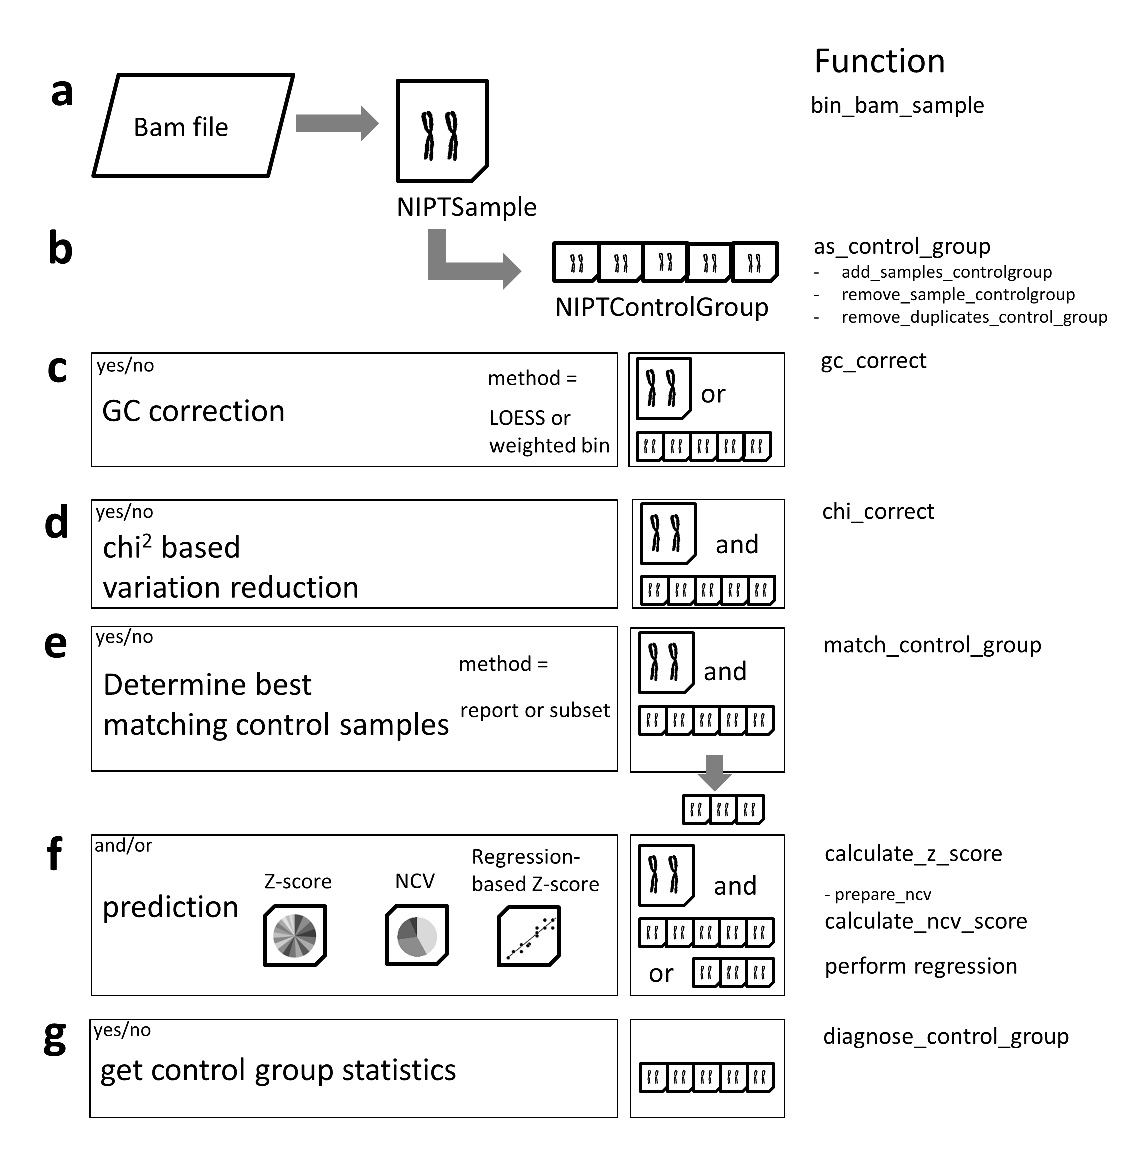
\includegraphics[width=1.0\linewidth]{img/NIPTeR_Fig1}
	\caption[Workflow and functions of NIPTeR]{Workflow and functions of NIPTeR. \textbf{a} A BAM file is transformed into an NIPTSample object; \textbf{b} a series of NIPTSample objects can then be transformed into an NIPTControlGroup object; \textbf{c} optional LOESS or weighted bin GC correction; \textbf{d} optional chi-squared-based variation reduction; \textbf{e} optional comparison of NIPTSample and NIPTControlGroup and possible selection of a subset that best-matches the control group samples; \textbf{f} three different prediction methods: Z-score, normalized chromosome value or regression-based Z-score; \textbf{g} optional check of control group statistics}
	\label{fig:Algorithms_NIPT_Fig1}
\end{figure}

NIPTeR analysis uses two core objects. 
The first object is NIPTSample, which contains the counts of aligned sequence reads in 50,000 bp bins for a specific sample. 
The second object is NIPTControlGroup, which contains a series of NIPTSamples for comparison. Users generate NIPTSample using the function bin\_bam\_sample, which needs a BAM file \cite{Li_2009} as input. 
The user can optionally select to count reads mapped to the forward and reverse strands separately, so that they can each be used as a separate predictor. 
The as\_control\_group function converts a series of NIPTSample objects into a NIPTControlGroup. 
Within NIPTeR, users can manage an existing NIPTControlGroup using the add\_samples\_controlgroup, remove\_sample\_controlgroup and remove\_duplicates\_controlgroup functions.

Both NIPTSample and NIPTControlGroup can undergo one or more variation reduction steps to adjust the bin read counts, either using the gc\_correct function for weighted bin GC correction \cite{Fan_2010} or LOESS GC correction \cite{Chen_2011} or the chi\_correct function for $\chi$2VR. 
Each NIPTSample object shows the correction status for the autosomes and the sex chromosomes separately and indicates which variation reduction methods have been performed (or that they are ‘uncorrected’). 
$\chi$2VR can be applied to uncorrected or GC-corrected samples, and makes use of a NIPTSample and a NIPTControlGroup having an identical correction status.

Using the fractions of reads mapped to the different chromosomes, trisomy prediction can be generated for a given NIPTSample based on the NIPTControlGroup using three different prediction algorithms: (1) calculate\_z\_score, which uses a standard Z-score \cite{Chiu_2008}; (2) calculate\_ncv\_score, which uses an NCV \cite{Sehnert_2011}; and (3) perform\_regression, which uses RBZ. 
All three trisomy prediction functions use NIPTControlGroup to calculate the expected fraction of reads on the chromosome of interest. 
For NCV, this calculation is done in a separate function, prepare\_ncv, because the calculation is time-intensive and only has to be performed once for each NIPTControlGroup. 
The prediction functions then compare the observed fraction of reads of the chromosome of interest in the NIPTSample with the expected fraction. 
In NCV and RBZ calculations, users have the option of excluding selected chromosomes as predictors. Since chromosomes 13, 18 and 21 are the most likely candidates for a trisomy, these are excluded by default, but users do have the option of including them. 
The functions prepare\_ncv and perform\_regression provide users the option of using a train and test set to prevent over-fitting the models they create.

In addition to providing Z-scores, the functions also produce control group statistics. 
The function match\_control\_group provides a Match QC score, a calculation that shows how well the sample fits within the control group based on the fraction of reads mapped to the different chromosomes, a measure that can be shown in a report. 
Alternately, users can select a subset of best-matching control samples as a sample-specific control group using the arguments mode = "report" or "subset". 
When a sample has an anomalously high Match QC score, the control samples being used are not suitable as a control group for the sample being analyzed. 
A second quality control function, diagnose\_control\_group, calculates Z-scores for all samples and chromosomes in a NIPTControlGroup as well as the mean, standard deviation and Shapiro-Wilk test of those Z-scores. 
This information can be used to curate the control group as explained in detail in Additional file 1.

\newpage

\section{Results}\label{Results}
\subsection{Workflow}
All these NIPTeR building blocks can be combined into an analysis workflow. For example, the NIPTeR workflow for the Fan \& Quake analysis \cite{Fan_2010}, using a weighted bin GC correction and a standard Z-score prediction for trisomy 21, and given a GC-corrected control group is: \\*

\fontfamily{pcr}\selectfont %pcr is the Courier font
\footnotesize
\noindent\textgreater\ NIPTsample \textless- bin\_bam\_sample(bam\_filepath = \\\indent "/Path/to/bam/sample.bam") \\
\textgreater\ NIPTsample\_gc \textless- gc\_correct(nipt\_object = NIPTsample, method = "bin") \\
\textgreater\ Zscore21\_NIPTsample \textless-  calculate\_z\_score(nipt\_sample = \\\indent NIPTsample\_gc, nipt\_control\_group = NIPTControlGroup\_gc, \\\indent chromo\_focus = 21) \\*
\fontfamily{mathpazo}\selectfont %back to original font

In addition, control group statistics and the match control of the sample to the control group can be performed: \\*

\fontfamily{pcr}\selectfont %pcr is the Courier font
\footnotesize %make text smaller
\noindent\textgreater\ NIPTcontrol\_diagnose - diagnose\_control\_group(nipt\_control\_group \\\indent= NIPT\_control\_group\_gc) \\
\textgreater\ MatchQC \textless- match\_control\_group(nipt\_sample = NIPTsample\_gc, \\\indent nipt\_control\_group = NIPT\_control\_group\_gc, mode = "report")
\fontfamily{mathpazo}\selectfont %back to original font
\normalsize %back to normal size

\subsection{Prediction and control group statistics}
The output formats of the calculate\_z\_score and calculate\_ncv\_score functions are similar. An example result of the main output reads: \\*

\fontfamily{pcr}\selectfont %pcr is the Courier font
\footnotesize %make text smaller
\noindent Zscore21\_NIPTsample\$sample\_Zscore \\
\noindent[1] 0.4575612 \medskip\\
Zscore21\_NIPTsample\$control\_group\_statistics \\
mean \hspace{20mm} SD \hspace{22mm} Shapiro\_P\_value  \\
1.380646e-02 \hspace{7mm} 7.184378e-05 \hspace{5mm} 9.498096e-01 \\*
\fontfamily{mathpazo}\selectfont %back to original font
\normalsize %back to normal size

Here, the Z-score is 0.45, which falls within the -3 to 3 range and leads to the conclusion that this sample does not have a trisomy 21. 
The control\_group\_statistics show the mean fraction of sequence reads mapping to chromosome 21 and the standard deviation (SD) of the fractions between the control samples. 
The Shapiro\_P\_value tests for control group normality, and control groups with a value above 0.05 can be considered to be normally distributed.



The output of perform\_regression is slightly different and gives four predictions based on different models when set to the default setting: \\*

\fontfamily{pcr}\selectfont %pcr is the Courier font
\tiny %make text much smaller
\noindent \hspace{16mm}	Prediction\_set\_1	\hspace{3mm} Prediction\_set\_2 \hspace{3mm} Prediction\_set\_3 \hspace{3mm} Prediction\_set\_4 \\
Z\_score\_sample  \hspace{1mm} 	0.695389767405796 \hspace{1mm} 0.436463271170429 \hspace{1mm} 0.437555582217223 \hspace{1mm} -0.268842730284741 \\
CV \hspace{13mm}	0.00536568258297721 0.00502335300817695 0.00483989627449594 0.00486660271957713 \\
cv\_types  \hspace{7mm}	Practical\_CV \hspace{7mm} Practical\_CV \hspace{7mm} Practical\_CV \hspace{6.3mm} Practical\_CV \\
P\_value\_shapiro \hspace{0mm}	0.430190936876808 \hspace{1mm} 0.844844184734285 \hspace{1.5mm} 0.478810106756347 \hspace{0.7mm} 0.606229054979589 \\
Pred\_chrom\footnote{In practice Pred\_chrom is written in full as: Predictor\_chromosomes. For layout purposes a shorthand is used here.} \hspace{4mm} 3F  1F  2R  7F \hspace{7mm}	3R  22F  1R  5R \hspace{7mm} 6R  10F  8R  17F \hspace{5mm} 20F  12F  19R  14F \\
Mean\_test\_set \hspace{2mm} 0.998406705791639 \hspace{1.2mm}	0.997692920712523 \hspace{1.7mm} 0.998044728541847 \hspace{1.1mm} 0.997802000172399 \\
CV\_train\_set \hspace{3mm} 0.00441576466562767 \hspace{0mm} 0.004609720864648 \hspace{0.9mm} 0.00479265227193279 \hspace{0.5mm}0.00492160650642337 \\*
\fontfamily{mathpazo}\selectfont %back to original font
\normalsize %back to normal size

Here, in addition to the RBZ, the coefficient of variation (CV) of the test set is given as a measure of control group variability. 
The type of CV is given as well, in which “Practical CV” is the true CV. If there is a risk of over-fitting the model on the control set, a theoretical CV is used. 
In addition to the Shapiro P value, perform\_regression reports the mean of the test set (which should be close to one) and the CV of the training set (based on which the chromosomes used to create the prediction model are selected), where reads mapped to the forward and reverse strands are used as separate entities.

\subsection{Quality control}
Using the diagnose\_control\_group function, control samples that have outliers that could hamper prediction can be detected. \\*


\fontfamily{pcr}\selectfont %pcr is the Courier font
\footnotesize %make text smaller
\noindent\textgreater\ NIPTcontrol\_diagnose\$abberant\_scores \medskip\\
\indent Chromosome \hspace{0mm} Sample\_name \hspace{0mm} Z\_score \\
1 \hspace{1mm} 17F \hspace{11mm} sample21 \hspace{4mm} 3.13281485801102 \\
2 \hspace{1mm} 1R  \hspace{13mm} sample21 \hspace{4mm} 3.1290608434065 \\
3 \hspace{1mm} 17R \hspace{11mm} sample21 \hspace{4mm} 3.33995848430216 \\
4 \hspace{1mm} 22R \hspace{11mm} sample24 \hspace{4mm} 3.08496372975161 \\
… \\
19 \hspace{1mm}8F \hspace{13mm}  sample21 \hspace{4mm} -3.85723794269498 \\
20 \hspace{1mm}5R \hspace{13mm}  sample21 \hspace{4mm} -3.16594249087773 \\
21 \hspace{1mm}16R\hspace{13mm}  sample21 \hspace{4mm} -3.5467264109158 \\*
\fontfamily{mathpazo}\selectfont %back to original font
\normalsize %back to normal size



This example shows that, for many chromosomes in sample 21 one or both of the strands have a Z-score higher than 3. 
This means that there is more variability in this sample than expected, pointing to a low quality sample. 
As explained in more detail in Additional file 1, we recommend that users remove samples that have more than one aberrant score (Z-score outside the -3 to 3 range) from the control group.

When looking at the individual Match QC scores of the GC corrected NIPTSample compared to the GC corrected NIPTControlGroup, the list of sum of squares of differences in chromosomal fractions of the test sample compared to each control sample is shown: \\*


\fontfamily{pcr}\selectfont %pcr is the Courier font
\footnotesize %make text smaller
\noindent \hspace{16mm} Sum\_of\_squares \\
sample86 \hspace{1mm} 1.919715e-07 \\
sample74 \hspace{1mm} 2.155461e-07 \\
… \\
sample40 \hspace{1mm} 1.089867e-06 \\
sample21 \hspace{1mm} 2.028651e-06 \\
\fontfamily{mathpazo}\selectfont %back to original font
\normalsize %back to normal size


In general, the lower the sum of squares, the more representative a control sample is for the test sample. 
The average of all sum of squares for an NIPTSample is the Match QC score. 
A Match QC score for a specific sample that falls outside 3 SD of the control group Match QC, indicates that the control group is not suitable for analysis of the sample.

Further examples and results can be found in the NIPTeR package vignette \cite{Johansson_2016} and the case report provided in Additional file 1. 
A demonstration of the NIPTeR GC-correction methods is given in Additional file 2 and a comparison of NIPTeR results with manual calculations is available for the $\chi$2VR in Additional file 3 and for the prediction methods and Match QC score in Additional file 4.

The NIPTeR package requires R 3.1.0 or higher, the stats and sets packages as available on CRAN, and the RSamtools and S4Vectors Bioconductor packages.

\subsection{Performance}
NIPTeR performance was tested on three different machines and operating systems (Additional file 5). 
Given a pre-processed control group of 100 samples, one sample was processed in 3 to 4 min (on average), including both GC correction and $\chi$2VR and using the Z-score and RBZ as prediction algorithms for chromosomes 13, 18 and 21. 
NCV analysis was performed in an additional 1 to 6 min using a maximum number of 6 to 9 chromosomes as denominator.

\section{Conclusion}\label{Conclusion}
NIPTeR allows for fast NIPT analysis and flexible workflow creation and includes variation correction and prediction algorithms as well as QC control. 
Algorithms used in NIPTeR are validated as described in Johansson and de Boer et al. (2017) \cite{Johansson_2017}. 
NIPTeR is available under the GNU GPL open source license and can be freely downloaded from https://github.com/molgenis/NIPTeR or CRAN.

\section{Availability and requirements}
\textbf{Project name:} NIPTeR.
\textbf{Project home page:} https://CRAN.R-project.org/package=NIPTeR
\textbf{Source page:} https://github.com/molgenis/NIPTeR
\textbf{Operating system(s):} Linux, MacOS, Windows.
\textbf{Programming language:} R.
\textbf{Other requirements:} R (3.1.0 or higher), RSamtools, sets, stats, S4Vectors.
\textbf{Licence:} GNU Lesser General Public License v3.0.
\textbf{Any restrictions to use by non-academics:} none

\section*{Acknowledgments}\label{Acknowledgments} 
We thank Kate Mc Intyre for editorial advice.

\section*{Authors’ contributions}
LJ is the main author. 
LJ and HdW conceived and designed the NIPTeR package. 
Together with FvD they developed and implemented the application. 
LJ, HdW, EdB and GtM designed and validated algorithms and implementation. 
RS, BS and MS were responsible for project administration and supervision. 
All authors read and approved the final version of this manuscript.

\section*{Ethics approval and consent to participate}
Not applicable.

\section*{Consent for publication}
Not applicable.

\section*{Competing interests}
The authors declare that they have no competing interests.

\section{Additional files}\label{Additional files}
Additional files can be accessed online: \\
\sloppy{https://bmcbioinformatics.biomedcentral.com/articles/10.1186/s12859-018-2557-8}



